% 编译使用xelatex编译一次

\documentclass[12pt, a4paper, oneside]{ctexart}
\usepackage{subcaption,listings,amsmath, amsthm, amssymb, bm, booktabs, color, framed,float, graphicx, hyperref, mathrsfs,minipage-marginpar}

\title{\textbf{数据库系统作业四}}
\author{2021113140符世博}
\date{}
\linespread{1.5}
\definecolor{shadecolor}{RGB}{241, 241, 255}
\newcounter{problemname}
\newenvironment{problem}{\begin{shaded}\stepcounter{problemname}\par\noindent\textbf{题目\arabic{problemname}. }}{\end{shaded}\par}
\newenvironment{solution}{\par\noindent\textbf{解答. }}{\par}
\newenvironment{note}{\par\noindent\textbf{题目\arabic{problemname}的注记. }}{\par}

\begin{document}
\maketitle

\begin{problem}
设有关系模式$R(A,B,C,D,E)$,$R$的函数关系依赖为

$F=\{B\rightarrow C,E\rightarrow D,D\rightarrow A,AC\rightarrow D,DC\rightarrow B\}$

\begin{enumerate}
    \item 求$(DC)_F^+$
    \item 求$R$的候选码
    \item 判断$R$属于第几范式
    \item 保持无损连接性和函数依赖,将$R$分解为$3NF$
\end{enumerate}

\end{problem}
\begin{solution}
    \begin{enumerate}
        \item $(DC)_F^+=\{ABCD\}$
        \item $BE$、$CE$
        \item 第一范式
        \item $R_1(E,D)\\R_2(E,B,C)\\R_3(D,A)$
    \end{enumerate}
\end{solution}

\begin{problem}
设有关系模式$R(A,B,C,D,G)$,$R$的函数关系依赖为

$F=\{AC\rightarrow B,C\rightarrow D,AC\rightarrow G,B\rightarrow C\}$

\begin{enumerate}
    \item 求$(AC)_F^+$
    \item 求$R$的候选码
    \item 判断$R$属于第几范式
    \item 保持无损连接性和函数依赖,将$R$分解为$3NF$
\end{enumerate}

\end{problem}
\begin{solution}
    \begin{enumerate}
        \item $(AC)_F^+=\{ABCDG\}$
        \item $AB$、$AC$
        \item 第一范式
        \item $R_1(A,B,C,G)\\R_2(C,D)$
    \end{enumerate}
\end{solution}

\begin{problem}
求F的最小依赖集

$F=\{AB\rightarrow C,D\rightarrow EG,C\rightarrow A,BE\rightarrow C,BC\rightarrow D,CG\rightarrow BD,ACD\rightarrow B,CE\rightarrow AG\}$

\end{problem}
\begin{solution}

    $F_1=\{AB\rightarrow C,D\rightarrow EG,BC\rightarrow D\}$

\end{solution}

\begin{problem}
有一个商品信息表

$Shop(SNo,INo,INum,DNo,DName)$

表中各属性含义为
\begin{table}[H]
    \centering
    \begin{tabular}{ccccc}
        \toprule[1.5pt]
        $SNo$ & $INo$ & $INum$ & $DNo$ & $DName$ \\
        \midrule[1pt]
        商店编号  & 商品编号  & 商品库存信息 & 部门编号  & 部门负责人   \\
        \bottomrule[1.5pt]
    \end{tabular}
\end{table}

这些数据有如下语义:

\begin{itemize}
    \item 每个商店的每种商品旨在该商店的一个部门销售
    \item 每个商店的每个部门只有一个部门负责人
    \item 每个商店的每种商品只有一个库存数量
\end{itemize}

\begin{enumerate}
    \item 根据上述语义写出关系$Shop$的函数依赖
    \item 找出关系$Shop$的候选码
    \item 判断关系$Shop$所达到的最高范式等级
    \item 如果关系$Shop$不属于$3NF$,将$Shop$分解为具有无损连接性和保持函数依赖的$3NF$
\end{enumerate}
\end{problem}
\begin{solution}

    \begin{enumerate}
        \item $F=\{SNp,INo\rightarrow DNo;SNo,DNo\rightarrow DName;SNo,INo\rightarrow INum\}$
        \item $\{SNo,INo\}$
        \item 第三范式
    \end{enumerate}

\end{solution}

\begin{problem}
利用线性hash方法对以下记录进行hash存储,在初始hash表中加入以下数字:

$18,25,27,36,48,56,61$

请画出添加以上所有元素后,最终的索引结构以及关键步骤(进行桶的线性增长时)的索引结构

注:线性hash表中最多容纳$nb\theta$个记录,$b=2$,$\theta=0.85$

初始哈希桶结构为下图

\begin{figure}[H]
    \centering
    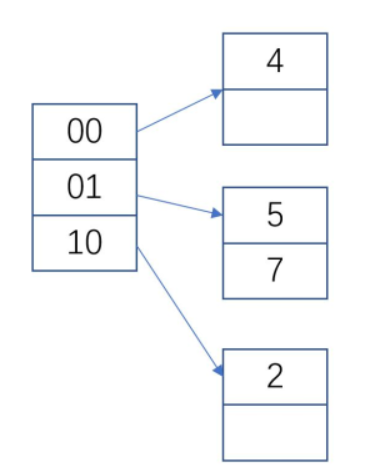
\includegraphics[width=0.50\textwidth]{figure/1.png}
\end{figure}

\end{problem}
\begin{solution}
    最终的索引结构如下图。

    \begin{figure}[H]
        \centering
        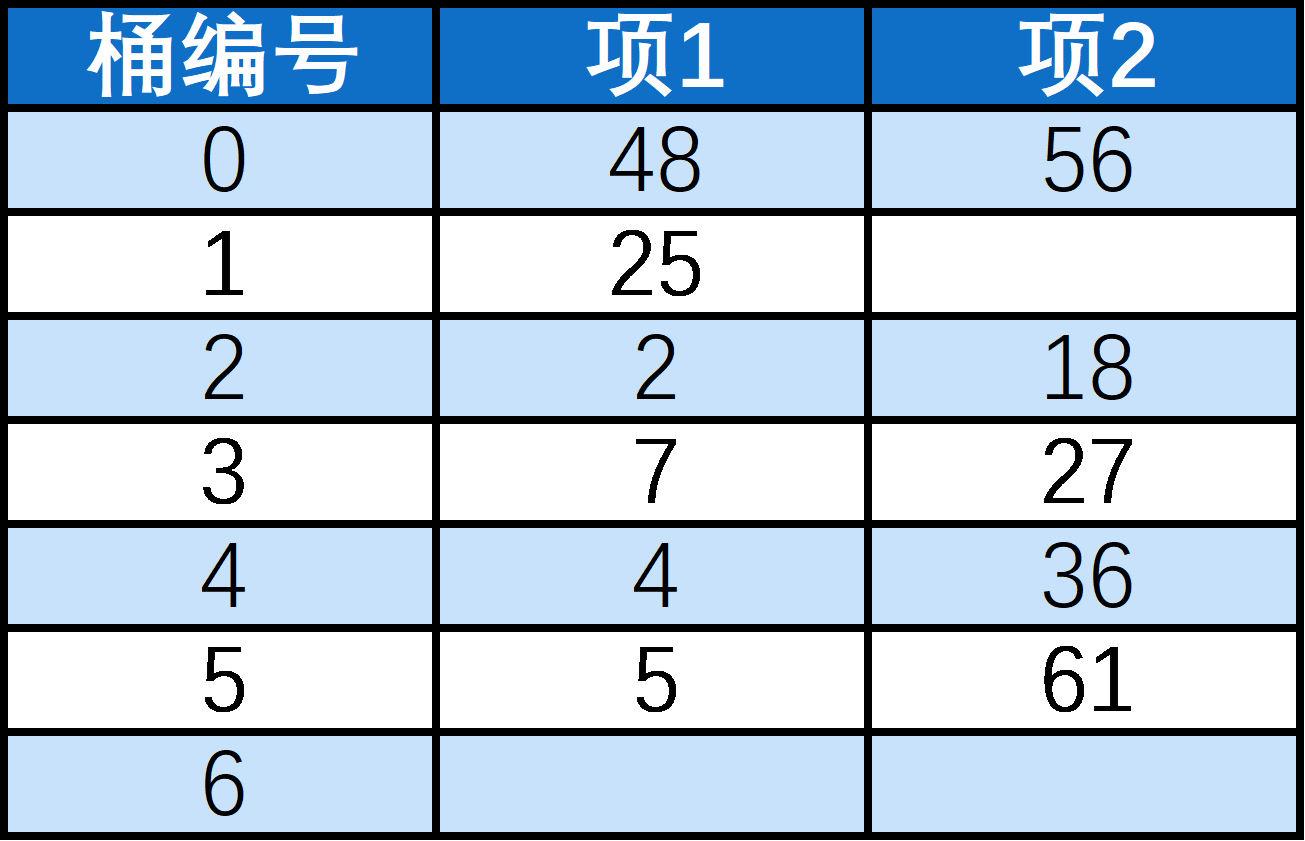
\includegraphics[width=0.50\textwidth]{figure/3.png}
    \end{figure}

    共发生了4次桶的线性增长,分别在插入25、27、48、61时,其变化如下图所示

    \begin{figure}[H]
        \centering
        \begin{minipage}[c]{0.45\textwidth}
            \centering
            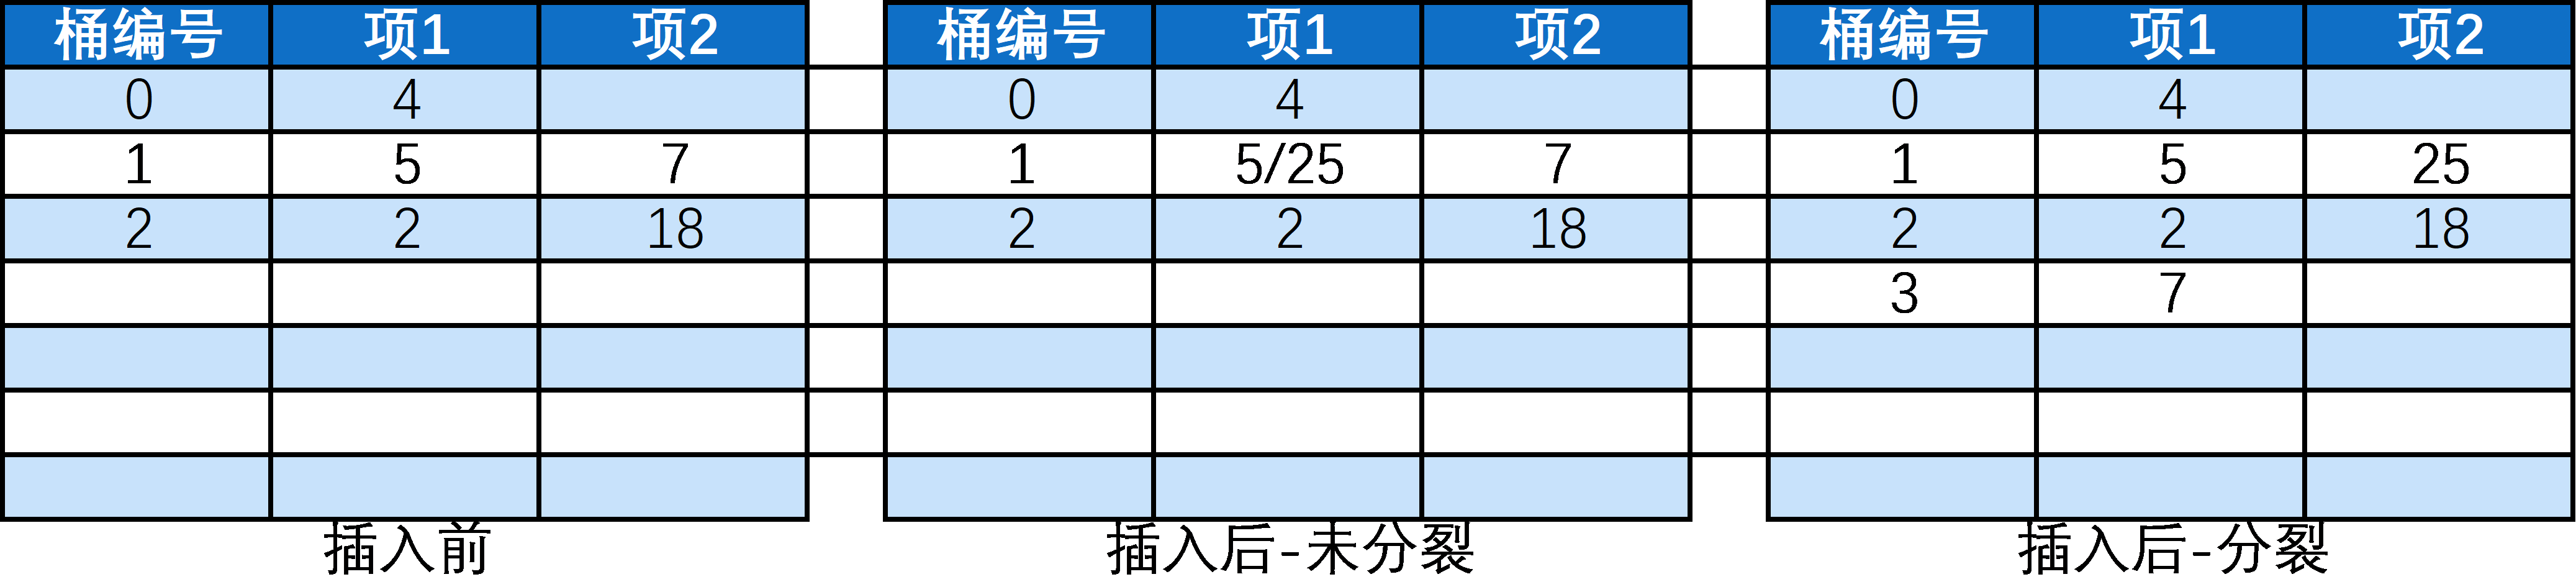
\includegraphics[width=0.95\textwidth]{figure/4-25.png}
            \subcaption{插入25}
        \end{minipage}
        \begin{minipage}[c]{0.45\textwidth}
            \centering
            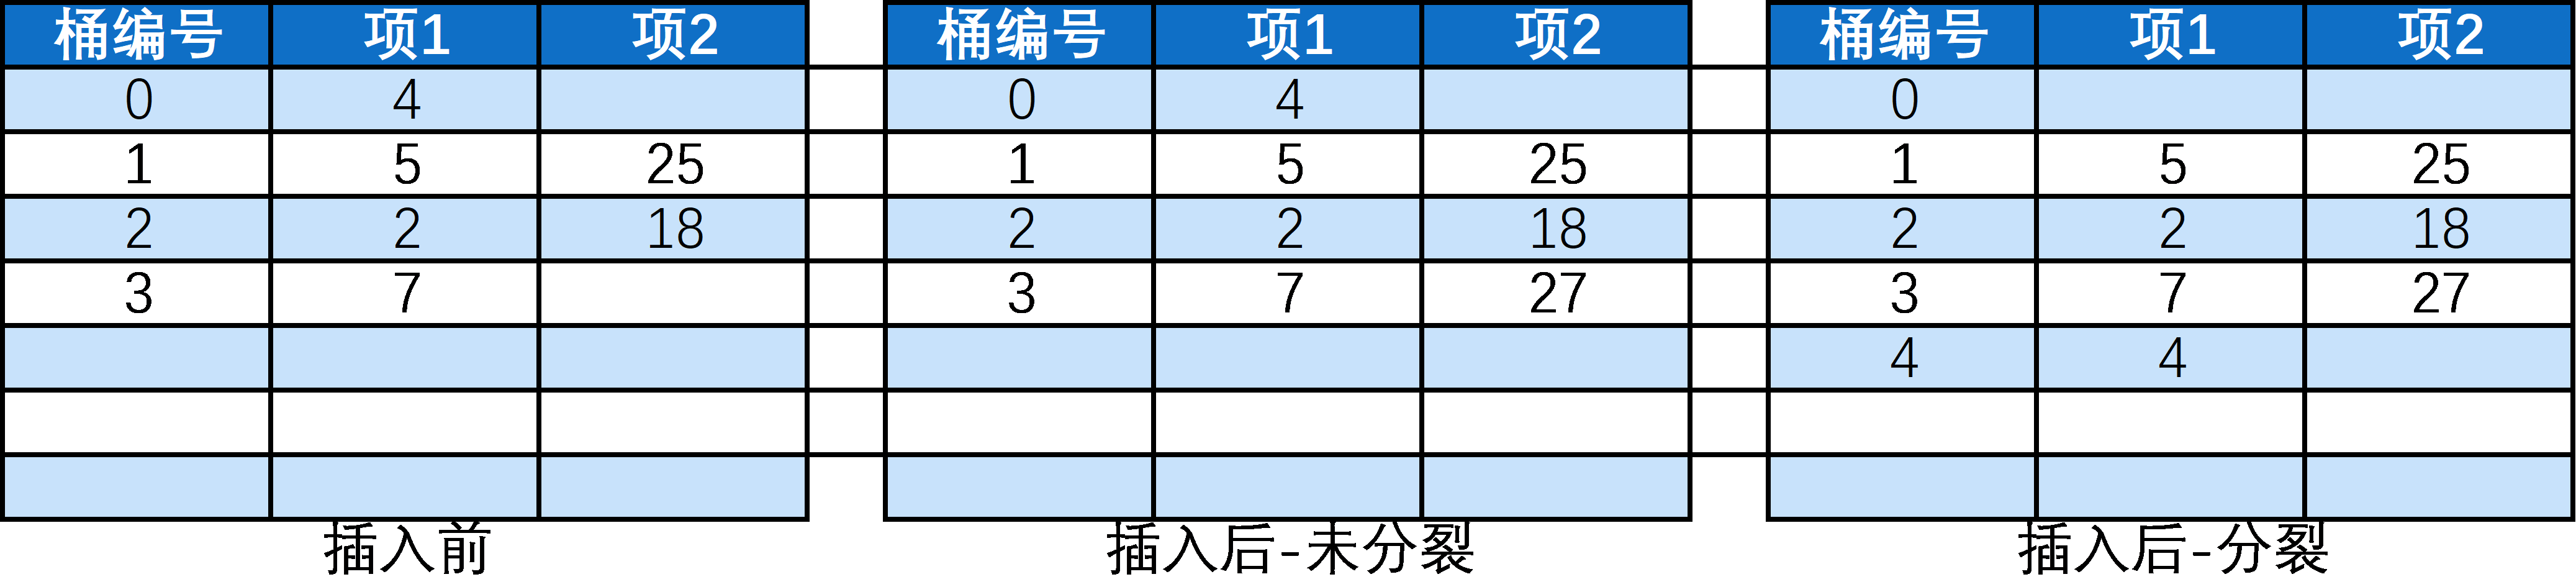
\includegraphics[width=0.95\textwidth]{figure/4-27.png}
            \subcaption{插入27}
        \end{minipage}

        \begin{minipage}[c]{0.45\textwidth}
            \centering
            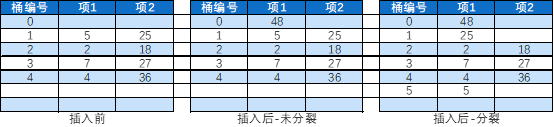
\includegraphics[width=0.95\textwidth]{figure/4-48.png}
            \subcaption{插入48}
        \end{minipage}
        \begin{minipage}[c]{0.45\textwidth}
            \centering
            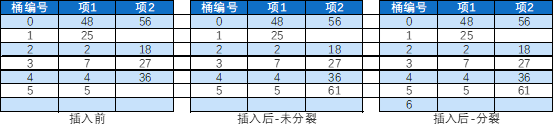
\includegraphics[width=0.95\textwidth]{figure/4-61.png}
            \subcaption{插入61}
        \end{minipage}
    \end{figure}
\end{solution}

\begin{problem}
已知一颗B+树,如下图所示

\begin{figure}[H]
    \centering
    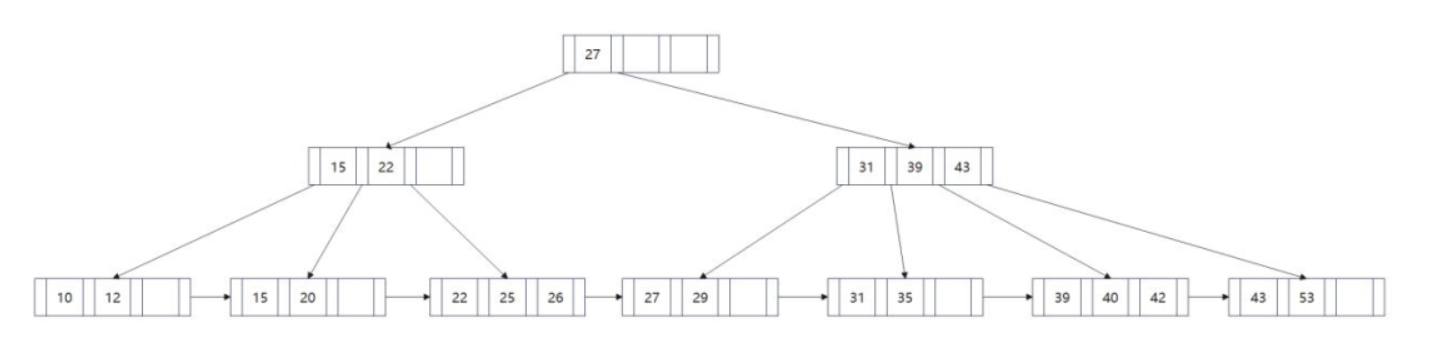
\includegraphics[width=0.95\textwidth]{figure/2.png}
\end{figure}

\begin{enumerate}
    \item 请画出插入23后所得到的新的B+树
    \item 请画出删除39后所得到的新的B+树
\end{enumerate}

\end{problem}
\begin{solution}

    \begin{figure}[H]
        \centering
        \begin{minipage}[c]{0.95\textwidth}
            \centering
            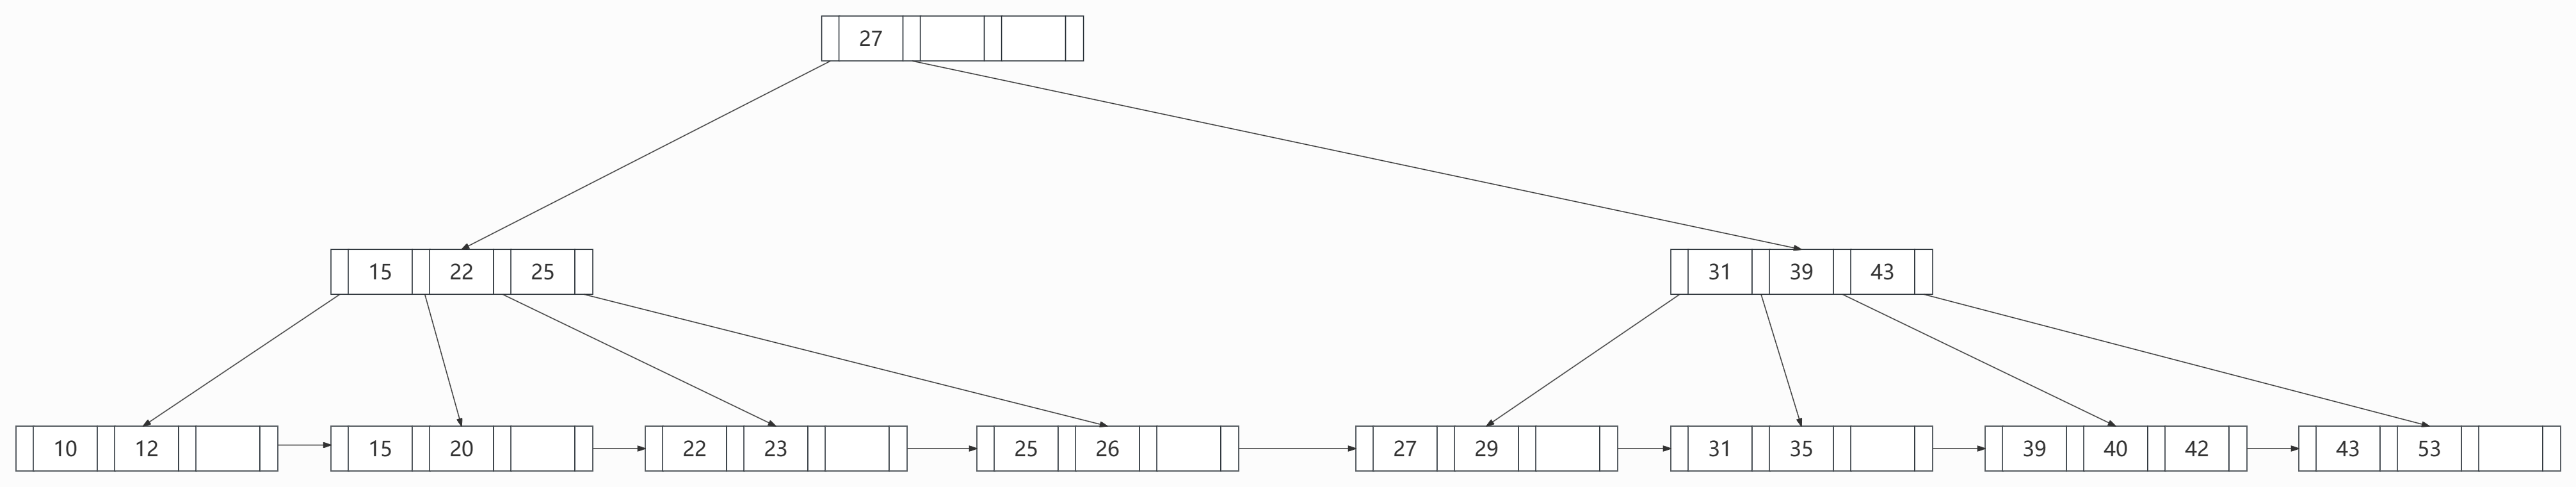
\includegraphics[width=0.95\textwidth]{figure/6-1.png}
            \subcaption{插入23后的B+树}
        \end{minipage}

        \begin{minipage}[c]{0.95\textwidth}
            \centering
            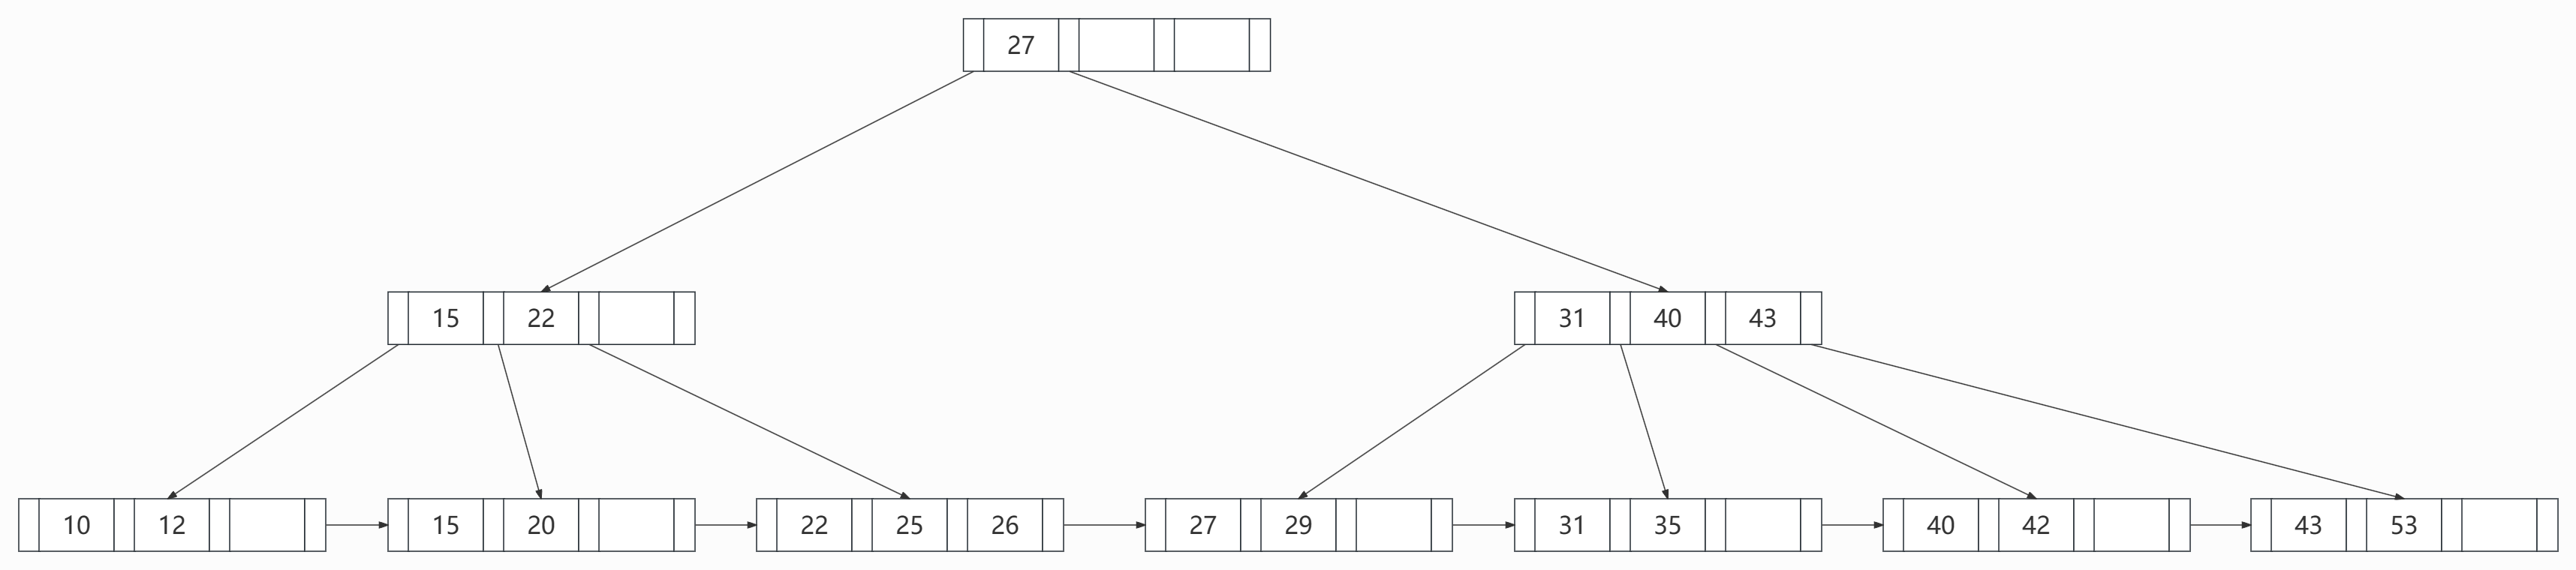
\includegraphics[width=0.95\textwidth]{figure/6-2.png}
            \subcaption{删除39后的B+树}
        \end{minipage}
    \end{figure}

\end{solution}

\begin{problem}
用下面的码集合建立一颗B+树:

$(2,3,5,7,11,17,19,23,29,31)$

假设树初始为空

\begin{enumerate}
    \item 按照升序添加这些值,阶数为3
    \item 按照降序添加这些值,阶数为3,对比与(1)中构造的树是否相同
\end{enumerate}

\end{problem}
\begin{solution}


    \begin{figure}[H]
        \centering
        \begin{minipage}[c]{0.95\textwidth}
            \centering
            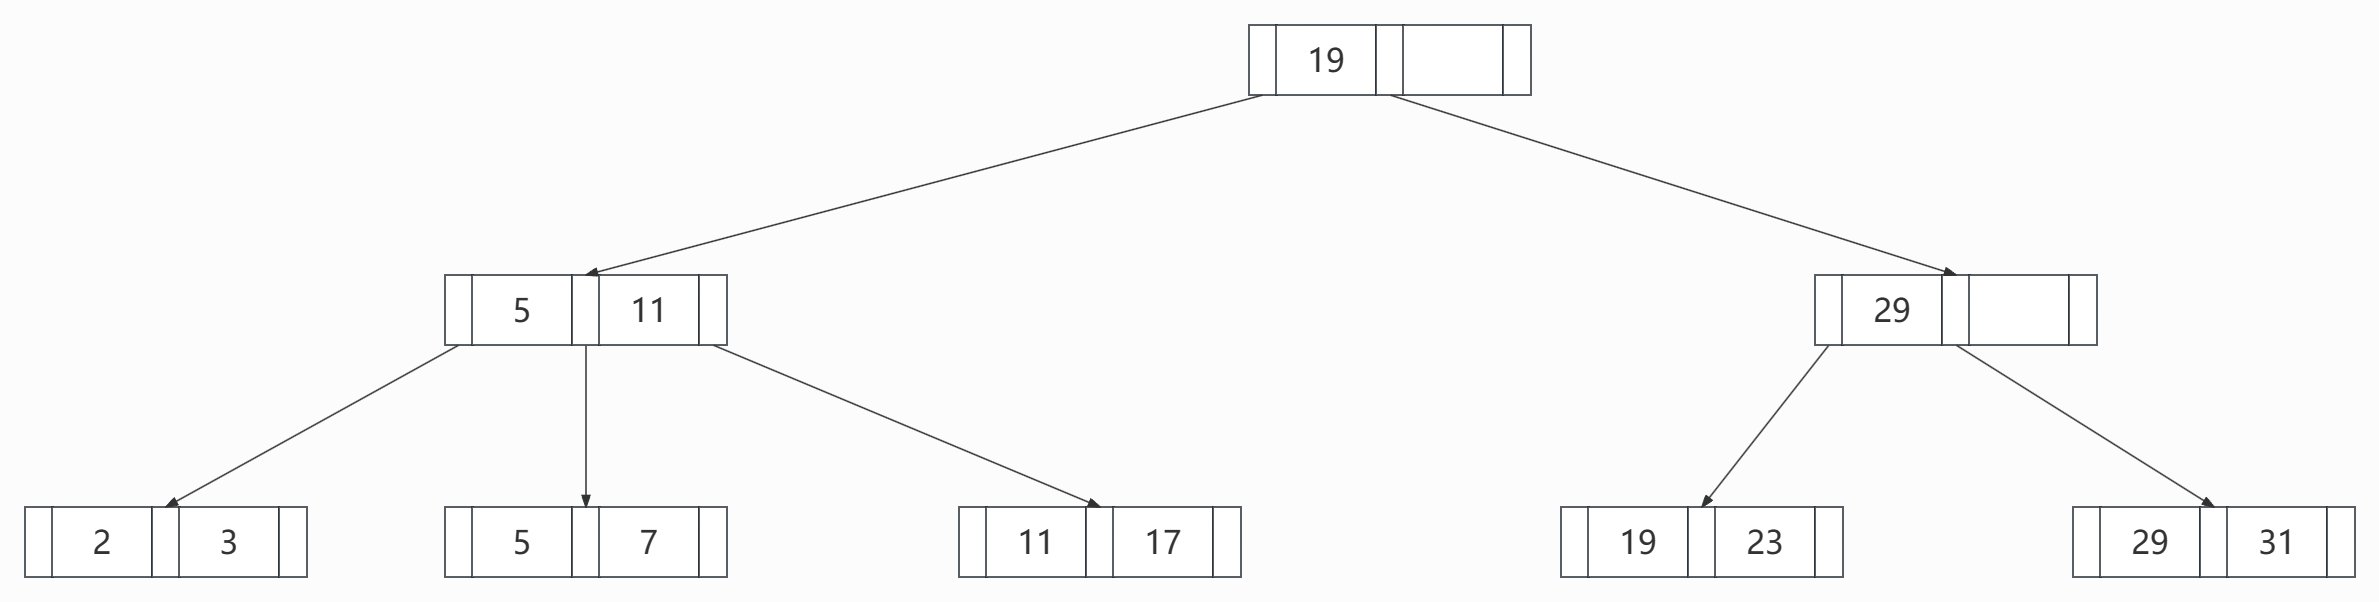
\includegraphics[width=0.95\textwidth]{figure/7-1.png}
            \subcaption{升序添加构造的B+树}
        \end{minipage}

        \begin{minipage}[c]{0.95\textwidth}
            \centering
            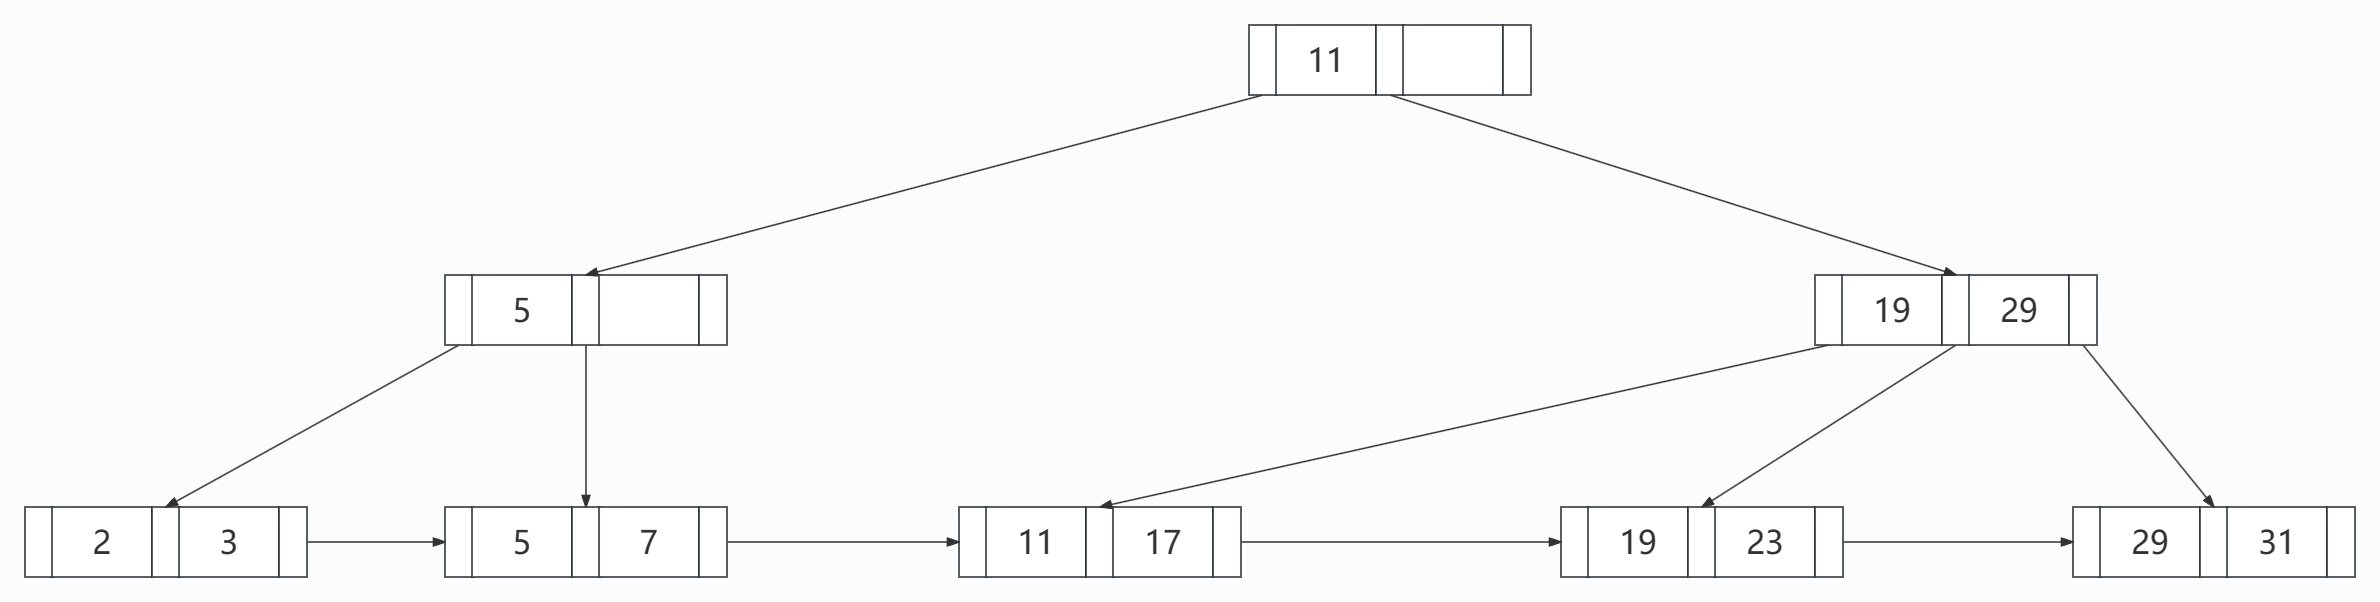
\includegraphics[width=0.95\textwidth]{figure/7-2.png}
            \subcaption{降序添加构造的B+树}
        \end{minipage}
    \end{figure}

    不相同

\end{solution}


\end{document}